% ============================================================
%  深圳大学实验报告模板（SZU Experiment Report Template）
% This template can be modified according to the specific requirements of your experiment or project.
% Produced by: Chao Fan and Kewei Ou, AI School of SZU
% ============================================================

\documentclass[a4paper,12pt]{article}

% ----------------------------
% 中文与字体支持
% ----------------------------
\usepackage{fontspec}    % 字体支持
\usepackage{xeCJK}       % 中文字体支持
\setCJKmainfont{Noto Serif CJK SC} % 设置中文字体（Overleaf自带Noto字体）

% ----------------------------
% 页面设置与常用宏包
% ----------------------------
\usepackage{geometry}    % 页面边距控制
\geometry{left=1in, right=1in, top=1in, bottom=1in}

\usepackage{longtable}   % 支持长表格
\usepackage{graphicx}    % 插入图片
\usepackage{fancyhdr}    % 页眉页脚控制
\usepackage{tikz}        % 绘制框线等图形
\usetikzlibrary{calc,shapes,arrows,positioning}    % 坐标计算、形状、箭头
\usepackage{verbatim}    % 显示代码块
\usepackage{float}       % 控制图片浮动位置（[H]参数）
\usepackage{hyperref}    % 超文本链接
\usepackage{xcolor}      % 颜色支持
\usepackage{enumitem}    % 列表控制

% ----------------------------
% 页眉页脚设置
% ----------------------------
\pagestyle{fancy}
\fancyhf{} % 清空默认页眉页脚
\fancyhead[L]{深圳大学实验报告} % 左侧页眉文字
\fancyhead[C]{} % 中间空
\fancyhead[R]{} % 右侧空

% ============================================================
%                      文档开始
% ============================================================

\begin{document}

% ============================================================
% 封面页
% ============================================================

\begin{titlepage}
    \centering
    \vspace*{2cm}
    \Huge{\textbf{深 \ 圳 \ 大 \ 学 \ 实 \ 验  \ 报 \ 告}}\\[1.5cm]
    
    \Large{课程名称：\underline{\makebox[8cm][c]{Python程序设计}}}\\[0.5cm]
    \Large{项目名称：\underline{\makebox[8cm][c]{《外星人入侵》小游戏}}}\\[0.5cm]
    \Large{学 \quad \quad 院：\underline{\makebox[8cm][c]{人工智能学院}}}\\[0.5cm]
    \Large{专 \quad \quad 业：\underline{\makebox[8cm][c]{计算机科学与技术（IEEE）}}}\\[0.5cm]
    \Large{指导教师：\underline{\makebox[8cm][c]{樊超、舒婷}}}\\[0.5cm]
    \Large
    报告人：\underline{\makebox[3.55cm][c]{朱明钊}}%
    \hspace{0.5cm}%
    学号：\underline{\makebox[2.8cm][c]{2024341011}}\\[0.5cm]
    \Large{实验时间：\underline{\makebox[8cm][c]{2025年11月12日-11月25日}}}\\[0.5cm]
    \Large{提交时间：\underline{\makebox[8cm][c]{2025年11月25日}}}\\[1.5cm]
    \vfill
    \Large{教务处制}
\end{titlepage}

\newpage

% ============================================================
% 正文部分
% ============================================================

\section{实验目的}

开发一款功能完整的2D太空射击游戏《外星人入侵》，通过项目实践掌握\textcolor{red}{Pygame游戏开发框架}、\textcolor{red}{面向对象编程设计}和\textcolor{red}{多系统协同架构}。

\section{实验内容}

\begin{enumerate}
    \item \textbf{核心玩法}：飞船控制、射击系统、碰撞检测和随机移动逻辑
    \item \textbf{扩展系统}：\textcolor{red}{升级、技能、装备、道具、大招、宝箱}六大系统
    \item \textbf{界面优化}：\textcolor{red}{开始界面、按钮美化、UI显示优化}
\end{enumerate}

\section{关键实现}

\subsection{模块化架构设计}

采用\textcolor{red}{面向对象设计}，将游戏拆分为25个模块，实现高内聚低耦合。游戏的完整UML类结构如图\ref{fig:class_diagram}所示：

\begin{figure}[H]
    \centering
    \includegraphics[width=0.95\linewidth]{uml_class_diagram.png}
    \caption{UML类关系图：展示所有类的完整结构、属性和方法，以及类之间的继承、组合、依赖关系。\textcolor{red}{核心特点}：①\texttt{AlienInvasion}作为主控制器，通过组合关系管理所有子系统；②游戏实体类（Ship、Alien、Bullet、Missile、LaserBullet等）统一继承自\texttt{pygame.sprite.Sprite}；③六大游戏系统（UpgradeSystem、SkillSystem、EquipmentManager、UltimateSkill、TreasureEffects、SoundManager）通过依赖关系与配置层（Settings、GameStats）交互；④UI层（Scoreboard、UpgradeMenu、StartScreen、ChestRewardUI）负责界面显示和用户交互。整体架构清晰，职责分离明确。}
    \label{fig:class_diagram}
\end{figure}

\textcolor{red}{架构优势}：\texttt{AlienInvasion}采用组合模式管理\textcolor{red}{6大系统}，各系统通过依赖注入实现解耦；游戏实体统一继承\texttt{Sprite}，利用pygame的碰撞检测机制；配置层（Settings、GameStats）为所有系统提供共享数据，保证数据一致性。

\subsection{系统交互流程}

游戏运行时，各系统通过主循环协调工作。图\ref{fig:system_flow}展示了完整的系统交互流程和方法调用链：

\begin{figure}[H]
    \centering
    \includegraphics[width=0.95\linewidth]{system_interaction_flow.png}
    \caption{系统交互流程图：详细展示游戏主循环中的方法调用流程和系统间的交互逻辑。\textcolor{red}{核心流程}包括：①\texttt{run\_game}主循环协调所有系统更新；②事件处理层（\texttt{\_check\_key\_events}）响应玩家输入，分发到技能系统、大招系统等；③物理更新层（\texttt{\_physics\_update}）处理碰撞检测、道具拾取、属性刷新；④游戏实体更新层（\texttt{sh.update}）同步更新玩家、单位、道具、效果等；⑤结算层处理经验获取、升级判定、连击统计等连锁反应；⑥渲染层（\texttt{\_update\_screen}）刷新所有UI元素。所有系统通过\textcolor{red}{事件驱动机制}实现异步解耦，保证游戏逻辑清晰和性能优化。}
    \label{fig:system_flow}
\end{figure}

\textcolor{red}{关键交互路径}：
\begin{itemize}[leftmargin=*,itemsep=0.05cm]
    \item \textbf{战斗循环}：击中外星人 → 经验获取 → 升级判定 → 显示升级菜单 → 属性提升
    \item \textbf{道具系统}：碰撞检测 → 道具拾取 → 效果激活 → 计时更新 → 效果失效
    \item \textbf{技能系统}：按键输入 → 技能判定 → 冷却计时 → 效果应用
    \item \textbf{关卡流程}：关卡完成 → 宝箱判定 → 奖励生成 → 装备/经验应用
\end{itemize}

\subsection{核心系统实现}

\textcolor{red}{六大系统协同}（详细实现逻辑见流程图\ref{fig:system_flow}）：
\begin{itemize}[leftmargin=*,itemsep=0.05cm]
    \item \textbf{升级系统}：击败外星人获得10点经验，升级后选择属性提升（攻击+10\%、射速-5\%、速度+8\%、生命+1、子弹+50）
    \item \textbf{技能系统}：5种主动技能（按键1-5触发）+ 4种被动技能（穿透、分裂、吸血、暴击），带冷却和持续时间机制
    \item \textbf{装备系统}：4种类型（武器/护甲/引擎/核心）× 4种品质（普通/稀有/史诗/传说），属性加成1.0x-2.0x
    \item \textbf{道具系统}：7种临时增益道具（激光、护盾、导弹、时间减缓、全屏爆炸、生命恢复、双倍分数），15\%掉落率
    \item \textbf{大招系统}：击败30个敌人充能100\%，释放4种随机大招（核爆、时间停止、流星雨、激光束）
    \item \textbf{宝箱系统}：每5关必得，其他关卡30\%概率，根据关卡等级动态生成品质
\end{itemize}

\section{实验结果}

项目已完成\textcolor{red}{完整游戏循环}和\textcolor{red}{8大扩展系统}（升级、技能、装备、道具、大招、宝箱、连击、音效），实现了\textcolor{red}{动态难度平衡}（外星人数量随关卡递增：12→40个）和\textcolor{red}{美观的UI界面}。图\ref{fig:gameplay}展示游戏运行效果。

\begin{figure}[H]
    \centering
    \includegraphics[width=0.92\linewidth]{gameplay.png}
    \caption{游戏实机画面：展示等级系统（Lv.3）、经验值条（EXP:140/144）、分数显示、大招充能条（20\%）等UI元素}
    \label{fig:gameplay}
\end{figure}

\textbf{代码统计}：25个模块文件，核心代码1148行，\textcolor{red}{关键方法均含中文注释}。通过UML类图（图\ref{fig:class_diagram}）和交互流程图（图\ref{fig:system_flow}）的设计，系统架构清晰，易于维护和扩展。

\section{讨论与改进}

\textcolor{red}{技术收获}：通过项目实践，掌握了Pygame游戏开发框架和面向对象编程设计模式。通过UML类图和交互流程图的设计（图\ref{fig:class_diagram}、图\ref{fig:system_flow}），深入理解了\textcolor{red}{事件驱动机制}、\textcolor{red}{系统解耦}和\textcolor{red}{模块化架构}的重要性。\textcolor{red}{项目亮点}：①25个模块职责清晰，高内聚低耦合；②六大系统属性完美叠加，平衡性良好；③UI界面美观，用户体验优化；④代码注释完善，遵循PEP 8规范。\textcolor{red}{改进方向}：可添加GitHub版本控制，扩展敌人类型和成就系统，增加游戏多样性。

\textbf{项目地址}：\href{https://github.com/your-username/alien_invasion}{\textcolor{blue}{GitHub项目链接}}

\newpage

% ============================================================
% 批阅与成绩评定页
% ============================================================

% 绘制正文外框（包含批阅区域）
\begin{tikzpicture}[remember picture, overlay]
  \draw[thick] 
    ($(current page.north west)+(2cm,-3cm)$) 
    rectangle 
    ($(current page.south east)+(-2cm,2.5cm)$);
\end{tikzpicture}

\vspace{1cm}

% 批阅区
\noindent \textbf{指导教师批阅意见：}

\vspace{5cm}

\hfill

\vspace{1cm}

\noindent \textbf{成绩评定：}

\vspace{2cm}

\hfill

\vspace{1cm}

\noindent \textbf{指导教师签字：}

\vspace{2cm}

\hfill

\vspace{1cm}

% 备注部分
\noindent \textbf{备注：}

\begin{itemize}
    \item 报告内的项目或内容设置，可根据实际情况加以调整和补充。
    \item 教师批改学生实验报告时间应在学生提交实验报告时间后 10 日内。
\end{itemize}

% ============================================================
%                      文档结束
% ============================================================

\end{document}

